\noindent\textbf{1.} Kết quả có thể tìm được từ quan hệ hình học:
\begin{equation}
  \label{eq:41}
  b=a+4R\cot\frac{\theta}{2}
\end{equation}

\noindent\textbf{2.} Các lực tác dụng lên thanh $C$ và $D$ được biểu diễn trên hình 4a và hình 4b. Đối với thanh $A$, phương trình cân bằng lực là:
\begin{equation}
  \label{eq:42}
  N_{1}+mg=N_{2}\cos\theta+f_{2}\sin\theta
\end{equation}
\begin{equation}
  \label{eq:43}
  f_{1}+f_{2}\cos\theta=N_{2}\sin\theta
\end{equation}
phương trình cân bằng momen đối với trụ quay đi qua khối tâm của thanh A là:
\begin{equation}
  \label{eq:44}
  f_{1}R=f_{2}R
\end{equation}
\begin{figure}[h]
  \centering
  \begin{minipage}{6cm}
    \centering
    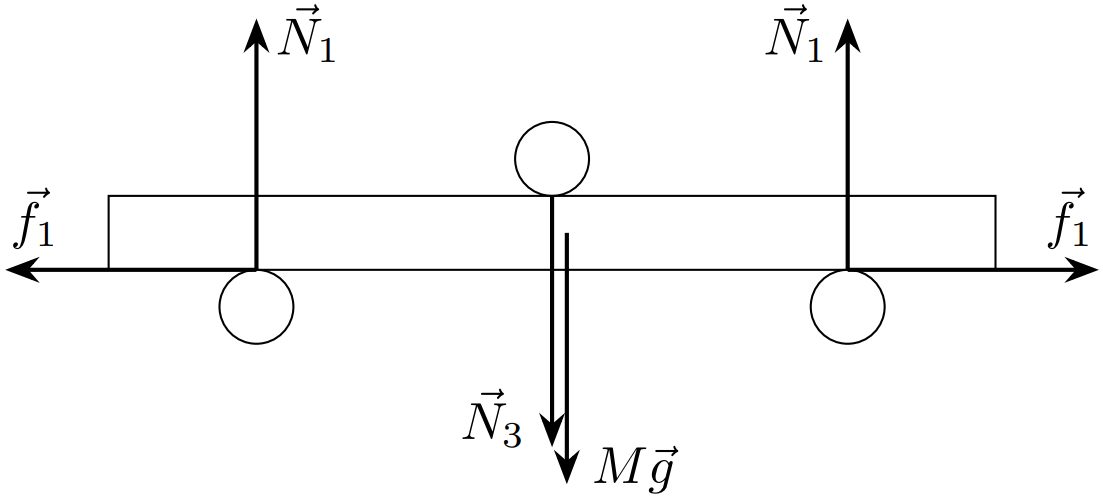
\includegraphics[width=1.4\textwidth]{images/Hinh 4a (S).png}
    \begin{center}
      \figurename{ 4a: Các lực tác dụng lên thanh $C$.}
    \end{center}
  \end{minipage}
  \hfil
  \begin{minipage}{6cm}
    \centering
    \includegraphics[width=0.8\textwidth]{images/Hình 4b (S).png}
    \begin{center}
      \figurename{ 4b: Các lực tác dụng lên thanh $D$.}
    \end{center}
  \end{minipage}
\end{figure}

\noindent đối với thanh $B$, phương trình cân bằng lực là:
\begin{equation}
  \label{eq:45}
  N_{3}=2N_{4}\cos\theta+mg
\end{equation}
đối với thanh $C$, phương trình cân bằng lực là:
\begin{equation}
  \label{eq:46}
  2N_{1}=N_{3}+Mg
\end{equation}
đối với thanh $D$, phương trình cân bằng lực là:
\begin{equation}
  \label{eq:47}
  N_{5}+N_{4}\cos\theta=N_{2}\cos\theta+f_{2}\sin\theta+Mg
\end{equation}
\begin{equation}
  \label{eq:48}
  f_{5}+N_{2}\sin\theta=N_{4}\sin\theta+f_{2}\cos\theta
\end{equation}
phương trình cân bằng momen đối với trục quay đi qua điểm tiếp xúc của thanh $D$ với mặt đất:
\begin{equation}
  \label{eq:49}
  N_{2}a+Mg\left(\frac{L}{2}\cos\theta-R\sin\theta\right)=N_{4}b+f_{2}2R
\end{equation}

\noindent\textbf{3.} Ta có:
\begin{equation}
  \label{eq:410}
  b=a+4R\cot\frac{\theta}{2}=\SI{24}{\centi\metre}
\end{equation}
từ \eqref{eq:42}, \eqref{eq:43} và \eqref{eq:44} ta có:
\begin{equation}
  \label{eq:411}
  f_{1}=f_{2}=\frac{\sin\theta}{1+\cos\theta}N_{2}
\end{equation}
\begin{equation}
  \label{eq:412}
  N_{1}+mg=N_{2}
\end{equation}
từ \eqref{eq:45} và \eqref{eq:46}:
\begin{equation}
  \label{eq:413}
  N_{1}=N_{4}\cos\theta+\frac{1}{2}(M+m)g
\end{equation}
thay \eqref{eq:411}, \eqref{eq:412}, \eqref{eq:413} vào \eqref{eq:49} ta có:
\begin{equation}
  \label{eq:414}
  (N_{1}+mg)a+Mg\left(\frac{L}{2}\cos\theta-R\sin\theta\right)=\left(N_{1}-\frac{1}{2}(M+m)g\right)\frac{b}{\cos\theta}+\frac{\sin}{1+\cos\theta}(N_{1}+mg)2R
\end{equation}
suy ra:
\begin{equation}
  \label{eq:415}
  N_{1}=\frac{mga+Mg\left(\dfrac{L}{2}\cos\theta-R\sin\theta\right)+\dfrac{1}{2}(M+m)g\frac{b}{\cos\theta}-\frac{\sin\theta}{1+\cos\theta}mg2R}{\dfrac{b}{\cos\theta}+\dfrac{\sin\theta}{1+\cos\theta}2R-a}=10,427mg
\end{equation}
từ \eqref{eq:411} và \eqref{eq:412} ta có:
\begin{align}
  \label{eq:416}
  f_{1}=f_{2} & =\frac{\sin\theta}{1+\cos\theta}(N_{1}+mg)                                                                                                                                                                                                                            \\\nonumber
              & =\frac{\sin\theta}{1+\cos\theta}\frac{Mg\left(\dfrac{L}{2}\cos\theta-R\sin\theta\right)+\dfrac{1}{2}(M+3m)g\dfrac{b}{\cos\theta}}{mga+Mg\left(\dfrac{L}{2}\cos\theta-R\sin\theta\right)+\dfrac{1}{2}(M+m)g\dfrac{b}{\cos\theta}-\dfrac{\sin\theta}{1+\cos\theta}mg2R} \\\nonumber
              & =4,733mg
\end{align}
để hệ duy trì được sự cân bằng:
\begin{equation}
  \label{eq:417}
  f_{1}\leqslant\mu N_{1},\quad f_{2}\leqslant\mu N_{2}
\end{equation}
suy ra:
\begin{align}
  \label{eq:418}
  \mu\geqslant\frac{f_{1}}{N_{1}} & =\frac{\sin\theta}{1+\cos\theta}\frac{Mg\left(\dfrac{L}{2}\cos\theta-R\sin\theta\right)+\dfrac{1}{2}(M+3m)g\dfrac{b}{\cos\theta}}{mga+Mg\left(\dfrac{L}{2}\cos\theta-R\sin\theta\right)+\dfrac{1}{2}(M+m)g\frac{b}{\cos\theta}-\dfrac{\sin\theta}{1+\cos\theta}mg2R} \\
  \nonumber                       & =0,454
\end{align}
từ \eqref{eq:42}, \eqref{eq:45}, \eqref{eq:46}, \eqref{eq:47} ta có:
\begin{equation}
  \label{eq:419}
  N_{5}=\frac{3}{2}(M+m)g=\frac{21}{2}mg
\end{equation}
từ \eqref{eq:48}, \eqref{eq:410}, \eqref{eq:411}, \eqref{eq:412} ta có:
\begin{equation}
  \label{eq:420}
  f_{5}=N_{1}\left(\tan\theta-\frac{\sin\theta}{1+\cos\theta}-\frac{1}{2}(M+m)g\tan\theta-mg\frac{\sin\theta}{1+\cos\theta}\right)=2,149mg
\end{equation}
điều kiện cân bằng:
\begin{equation}
  f_{5}\leqslant\mu' N_{5}
\end{equation}
suy ra:
\begin{equation}
  \label{eq:422}
  \mu'\geqslant\frac{f_{5}}{N_{5}}=\frac{2N_{1}}{3(M+m)g}\left(\tan\theta-\frac{\sin\theta}{1+\cos\theta}\right)-\frac{1}{3}\tan\theta-\frac{2m}{3(M+m)}\frac{\sin\theta}{1+\cos\theta}=0,209
\end{equation}
